%%%%%%%%%%%%%%%%%%%%%%%%%%%%%%%%%%%%%%%%%%%%%%%%%%%%%%%%%%%%%%%%%%%%%%
% Problem statement
\begin{statement}[
  problempoints=110,
  timelimit=1 sekunda,
  memorylimit=512 MiB,
]{Zvijezda}

%\setlength\intextsep{-0.1cm}
%\begin{wrapfigure}[3]{r}{0.22\textwidth}
%\centering
%\includegraphics[width=0.22\textwidth]{img/computer.png}
%\end{wrapfigure}

Budući da je štrajk i dalje aktivan, Mirko i Slavko vrijeme provode igrajući se
s $N$-terokutima i gledajući novu sezonu Života na vagi. Mirko je nedavno
nacrtao konveksan $N$-terkout s parnim brojem stranica, a Slavko je zatim
kroz parove nasuprotnih stranica (dvije stranice su nasuprotne ako se između
njih nalazi $\frac{N}{2}-1$ stranica) nacrtao pravce te obojio dio ravnine
koji se nalazi između njih i koji sadrži $N$-terkout. Tada je Mirko u ravninu
postavio $Q$ točaka i pitao Slavka da mu za svaku točku kaže nalazi li se na
obojenom ili neobojenom dijelu ravnine.

Budući da uskoro počinje najnovija epizoda Života na vagi, Slavko nema vremena
pronaći odgovor na Mirkove upite te vas moli da mu pomognete.

%%%%%%%%%%%%%%%%%%%%%%%%%%%%%%%%%%%%%%%%%%%%%%%%%%%%%%%%%%%%%%%%%%%%%%
% Input
\subsection*{Ulazni podaci}
U prvom retku nalazi se broj $T$ pomoću kojeg određujemo Mirkove upite. Broj
$T$ može biti samo $0$ ili $1$.

U drugom retku je paran prirodan broj $N$ iz teksta zadatka.

U svakom od sljedećih $N$ redaka su dva cijela broja $X_i$, $Y_i$
$(0 \le |Xi|, |Yi| \le 10^9$
koji predstavljaju neki od vrhova mnogokuta. Možete pretpostaviti
da su vrhovi $N$-terokuta zadani u smjeru suprotnom od kazaljke na satu i da ne
postoje dvije uzastopne paralelne dužine.

U sljedećem je retku prirodan broj $Q$ koji označava broj Mirkovih upita.

U svakom od sljedećih $Q$ redaka su dva cijela broja $A_i$, $B_i$
$(0 \le |Ai|, |Bi| \le 2\cdot10^{18})$ koji predstavljaju parametre kojima
određujemo točku Mirkova $i$-tog upita.

Neka je $X_i$ jednak broju točaka među prvih $i$ (uključivo) Mirkovih upita
koje leže na obojenom dijelu ravnine. Dakako, $X_0=0$. Točka koja predstavlja
$i$-ti Mirkov upit je tada:
\[P_i = (A_i \oplus (T \cdot X_{i-1}^{3}), B_i \oplus (T \cdot X_{i-1}^{3}))\]
gdje znak $\oplus$ predstavlja bitovni xor (isključivo ili).

%%%%%%%%%%%%%%%%%%%%%%%%%%%%%%%%%%%%%%%%%%%%%%%%%%%%%%%%%%%%%%%%%%%%%%
% Output
\subsection*{Izlazni podaci}
U $i$-tom od $Q$ redova potrebno je ispisati \texttt{"DA"} (bez navodnika) ako
$i$-ta točka leži na obojenom dijelu ravnine, a inače je potrebno ispisati
\texttt{"NE"} (bez navodnika).

%%%%%%%%%%%%%%%%%%%%%%%%%%%%%%%%%%%%%%%%%%%%%%%%%%%%%%%%%%%%%%%%%%%%%%
% Scoring
\subsection*{Bodovanje}
{\renewcommand{\arraystretch}{1.4}
  \setlength{\tabcolsep}{6pt}
  \begin{tabular}{ccl}
 Podzadatak & Broj bodova & Ograničenja \\ \midrule
  1 & 20 & $1 \le N, Q \le 2000$, $T = 0$ \\
  2 & 30 & $1 \le N, Q \le 10^5$, $T = 0$ \\
  3 & 60 & $1 \le N, Q \le 10^5$, $T = 1$
\end{tabular}}

%%%%%%%%%%%%%%%%%%%%%%%%%%%%%%%%%%%%%%%%%%%%%%%%%%%%%%%%%%%%%%%%%%%%%%
% Examples
\subsection*{Probni primjeri}
\begin{tabularx}{\textwidth}{X'X'X}
\sampleinputs{test/zvijezda.dummy.in.1}{test/zvijezda.dummy.out.1} &
\sampleinputs{test/zvijezda.dummy.in.2}{test/zvijezda.dummy.out.2} &
\sampleinputs{test/zvijezda.dummy.in.3}{test/zvijezda.dummy.out.3}
\end{tabularx}

\textbf{Pojašnjenje drugog probnog primjera:}
\begin{figure}[H]
\centering
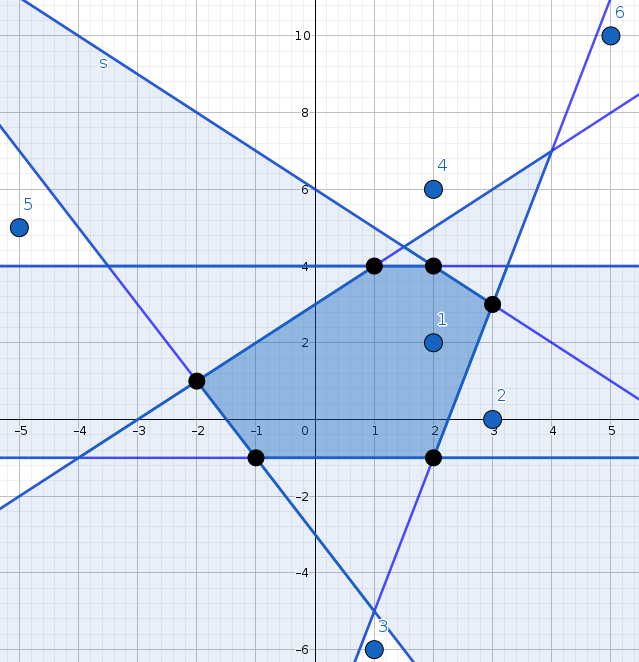
\includegraphics[width=0.5\textwidth]{img/zvijezda_clar.png}
\end{figure}

\textbf{Pojašnjenje trećeg probnog primjera:}
Obojena površina je jednaka kao i u drugom probnom primjeru, a koordinate
točaka Mirkovih upita su redom: $(2, 2)$, $(2, 1)$, $(9, -14)$, $(25, 29)$,
$(-32, 30)$ i $(30, 17)$.

%%%%%%%%%%%%%%%%%%%%%%%%%%%%%%%%%%%%%%%%%%%%%%%%%%%%%%%%%%%%%%%%%%%%%%
% We're done
\end{statement}

%%% Local Variables:
%%% mode: latex
%%% mode: flyspell
%%% ispell-local-dictionary: "croatian"
%%% TeX-master: "../hio.tex"
%%% End:
